\documentclass[12pt]{article}
\usepackage[top=1in,left=1in, right = 1in, footskip=1in]{geometry}

\usepackage{graphicx}
%\usepackage{adjustbox}

\newcommand{\eref}[1]{(\ref{eq:#1})}
\newcommand{\fref}[1]{Fig.~\ref{fig:#1}}
\newcommand{\Fref}[1]{Fig.~\ref{fig:#1}}
\newcommand{\sref}[1]{Sec.~\ref{#1}}
\newcommand{\frange}[2]{Fig.~\ref{fig:#1}--\ref{fig:#2}}
\newcommand{\tref}[1]{Table~\ref{tab:#1}}
\newcommand{\tlab}[1]{\label{tab:#1}}
\newcommand{\seminar}{SE\mbox{$^m$}I\mbox{$^n$}R}

\usepackage{amsthm}
\usepackage{amsmath}
\usepackage{amssymb}
\usepackage{amsfonts}

\usepackage{lineno}
%\linenumbers

\usepackage[pdfencoding=auto, psdextra]{hyperref}

\bibliographystyle{chicago}
\usepackage{natbib}
\date{\today}

\usepackage{xspace}
\newcommand*{\ie}{i.e.\@\xspace}

\usepackage{color}

\newcommand{\Rx}[1]{\ensuremath{{\mathcal R}_{#1}}} 
\newcommand{\Ro}{\Rx{0}}
\newcommand{\RR}{\ensuremath{{\mathcal R}}}
\newcommand{\Rhat}{\ensuremath{{\hat\RR}}}
\newcommand{\tsub}[2]{#1_{{\textrm{\tiny #2}}}}

\newcommand{\comment}[3]{\textcolor{#1}{\textbf{[#2: }\textsl{#3}\textbf{]}}}
\newcommand{\jd}[1]{\comment{cyan}{JD}{#1}}
\newcommand{\swp}[1]{\comment{magenta}{SWP}{#1}}
\newcommand{\dc}[1]{\comment{blue}{DC}{#1}}
\newcommand{\hotcomment}[1]{\comment{red}{HOT}{#1}}

\newcommand{\jdnew}{\jd{NEW}}
\newcommand{\jddel}[1]{\jd{DELETE: #1}}

\begin{document}

\begin{flushleft}{
	\Large
	\textbf\newline{
		Antigenic evolution of influenza under non-pharmaceutical interventions
	}
}
\newline
\\
\end{flushleft} 

\tableofcontents

\pagebreak

\section{Methods summary}

Here, we use a modified version of the multi-strain model developed by \cite{gog2002dynamics}:
\begin{align}
\dot{S_i} &= \mu - \sum_j \beta(t) S_i \sigma_{ij} I_j - \mu S_i\\
\dot{I_1} &= \beta(t) S_1 I_1 - \gamma I_1 - \mu I_1 - m I_1\\
\dot{I_i} &= \beta(t) S_i I_i - \gamma I_i - \mu I_i - m I_i + mI_{i-1}\\
\dot{I_n} &= \beta(t) S_n I_n - \gamma I_n - \mu I_n + mI_{n-1}\\
\end{align}
For simplicity, we assume that evolution causes strains to evolve in one direction ($i-1$ to $i$).
Here, $\sigma_{ij}$ determines the strength of cross immunity:
\begin{equation}
\sigma_{ij} = \exp\left(-((i-j)/d)^2\right).
\end{equation}
The transmission rate is assumed to follow a sinusoidal shape:
\begin{equation}
\beta(t) = b_0 (1 + b_1 \cos(2 \pi t)).
\end{equation}
We simulate the model for 20 years for it to allow the system to reach equilibrium and introduce intervention that reduces the transmission rate by a fixed amount.
Parameters are chosen roughly based on \cite{gog2002dynamics} such that the pre-intervention dynamics exhibit annual cycles.

\pagebreak

\section{6 month control}

\begin{figure}[!h]
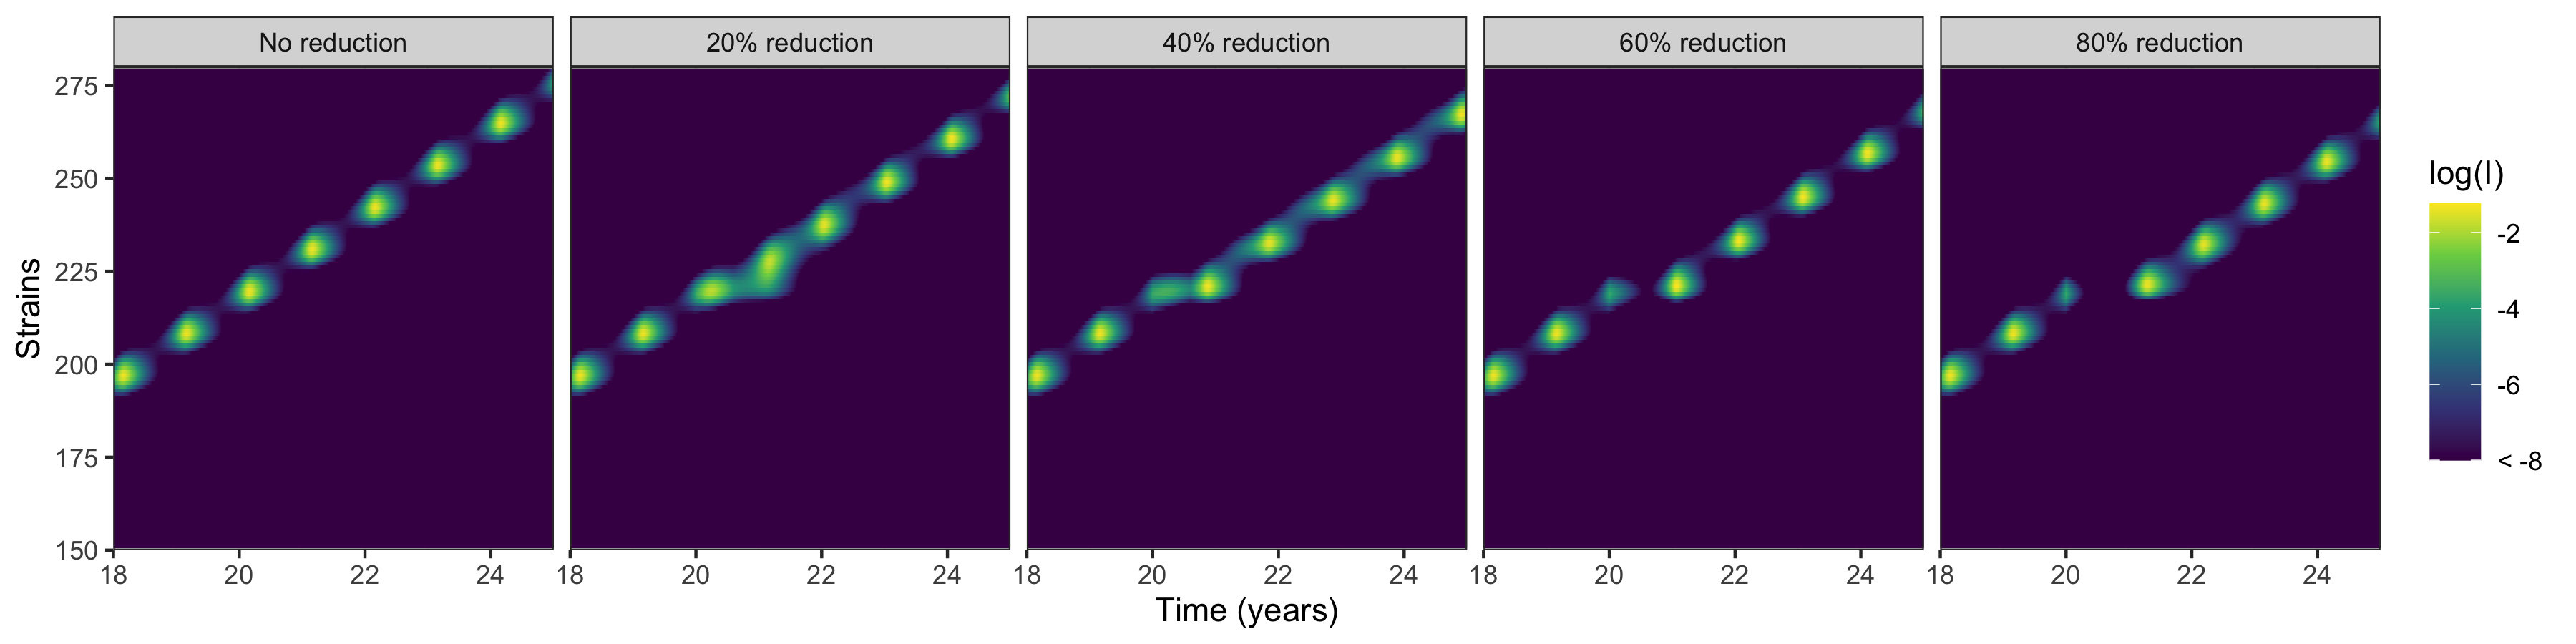
\includegraphics[width=\textwidth]{../figure/figure_flu_ode_6month_1.pdf}
\caption{
\textbf{Impact of reduction in transmission rate on epidemic dynamics.}
Under strong intervention ($>40\%$), reduction in transmission ``stops'' evolution, and therefore the evolution continues from where we left off when the intervention is lifted.
Under moderate intervention ($20\%$), we still get a moderate outbreak, which induces selective pressure on new strains and increases strain diversity.
This is because a moderate outbreak insufficiently depletes the susceptible pool, allowing for non-dominant strains to persist.
}
\end{figure}

\pagebreak

\begin{figure}[!h]
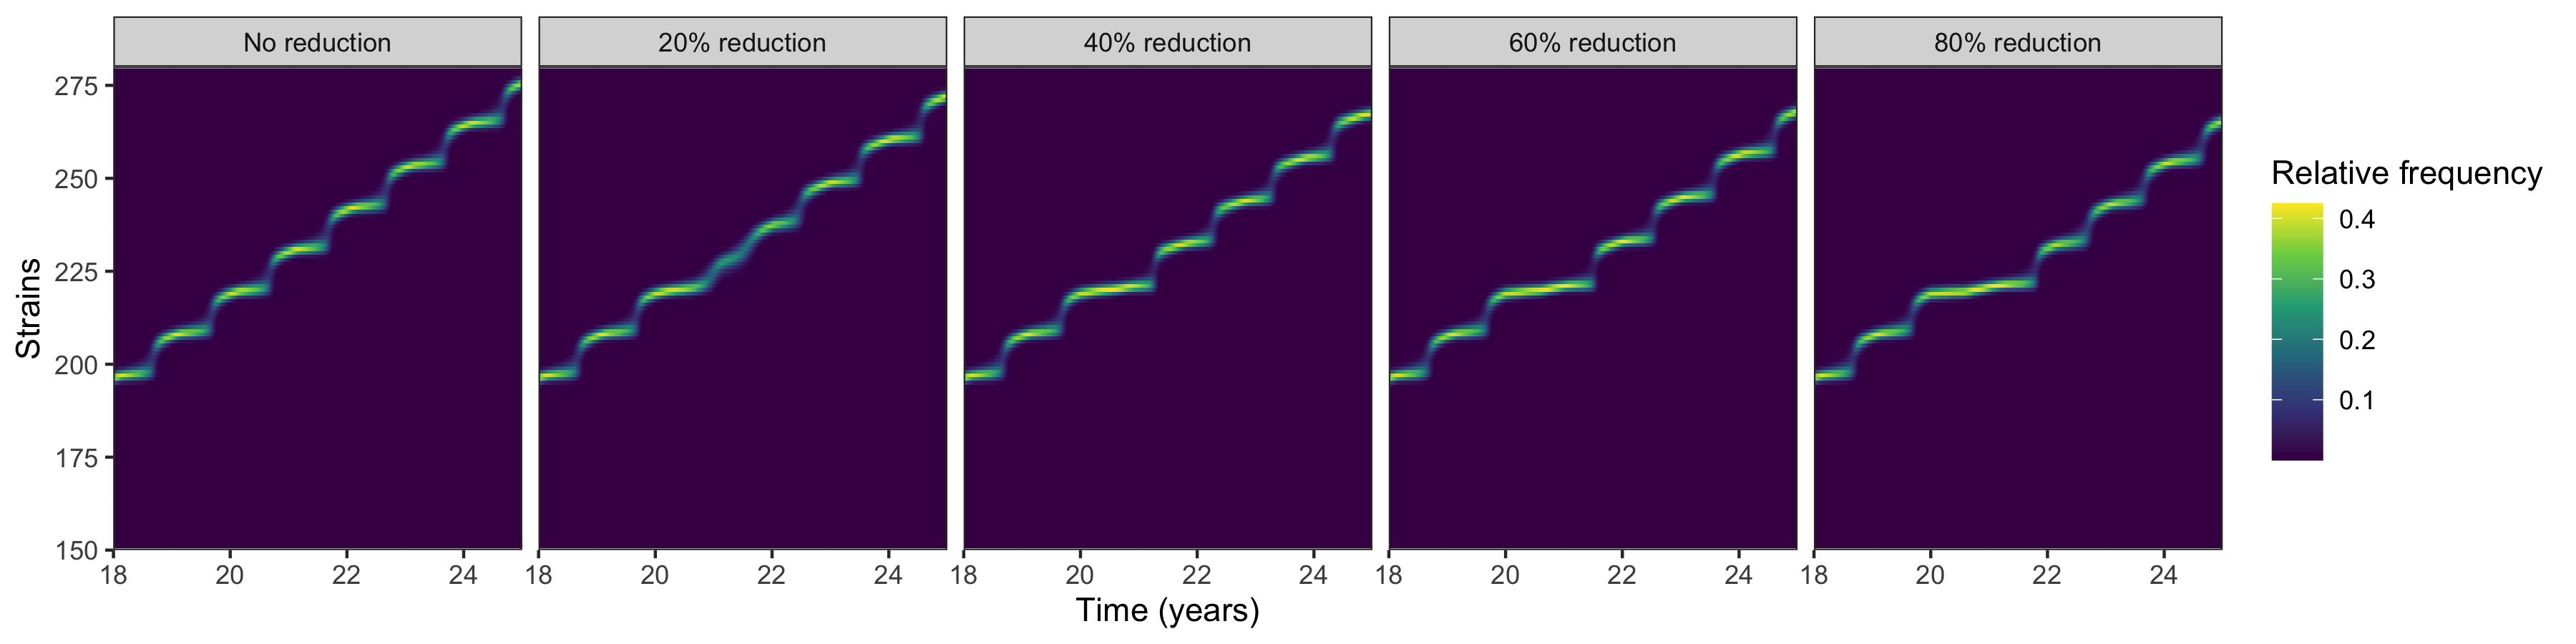
\includegraphics[width=\textwidth]{../figure/figure_flu_ode_6month_2.pdf}
\caption{
\textbf{Impact of reduction in transmission rate on relative frequencies of each strain.}
Here, we use same simulations as Figure 1, but show relative frequencies (i.e., $I_i/\sum_j I_j$) instead of absolute prevalence ($I_i$).
This figure clearly illustrates how strong interventions can stop the evolution.
Note that interventions may lead to unexpected transient dynamics in evolution (see $20\%$ and $60\%$ where we see a continuous changes in dominant strains, rather than a step-like evolution observed in other scenarios).
}
\end{figure}


\pagebreak

\begin{figure}[!h]
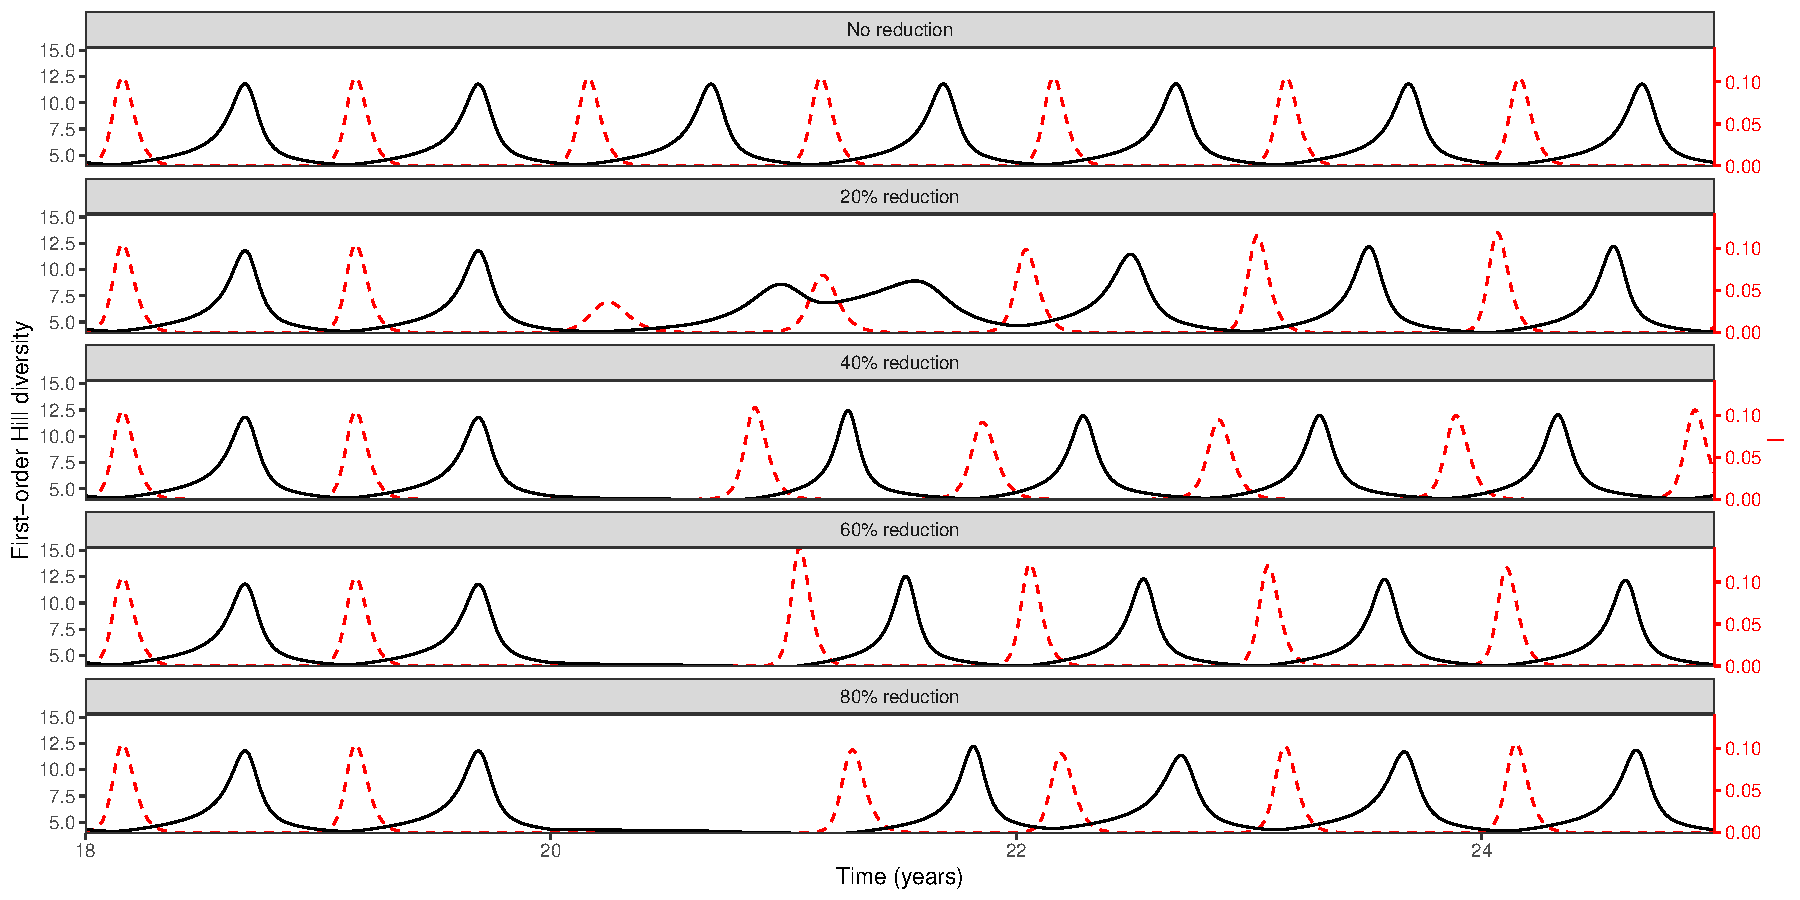
\includegraphics[width=\textwidth]{../figure/figure_flu_ode_6month_4.pdf}
\caption{
\textbf{Impact of reduction in transmission rate on strain diversity.}
Black lines represent the first order Hill diversity.
Red lines represent total prevalence $I = \sum_j I_j$.
Here, we see that strain diversity increases during off-season under regular dynamics:
When the epidemic is spreading, dominant strains burn through the susceptible pool and prevent other strains from spreading; note there is weak selective pressure during this period since susceptibility is relatively high.
As the epidemic subsides, other strains that have selective advantage persist and the diversity increases.
Epidemic interventions can induce transient effects, which generate small outbreaks (see $20\%$ and $60\%$) that cause some selective pressure and allow for high diversity to be maintained.
}
\end{figure}


\pagebreak

\begin{figure}[!h]
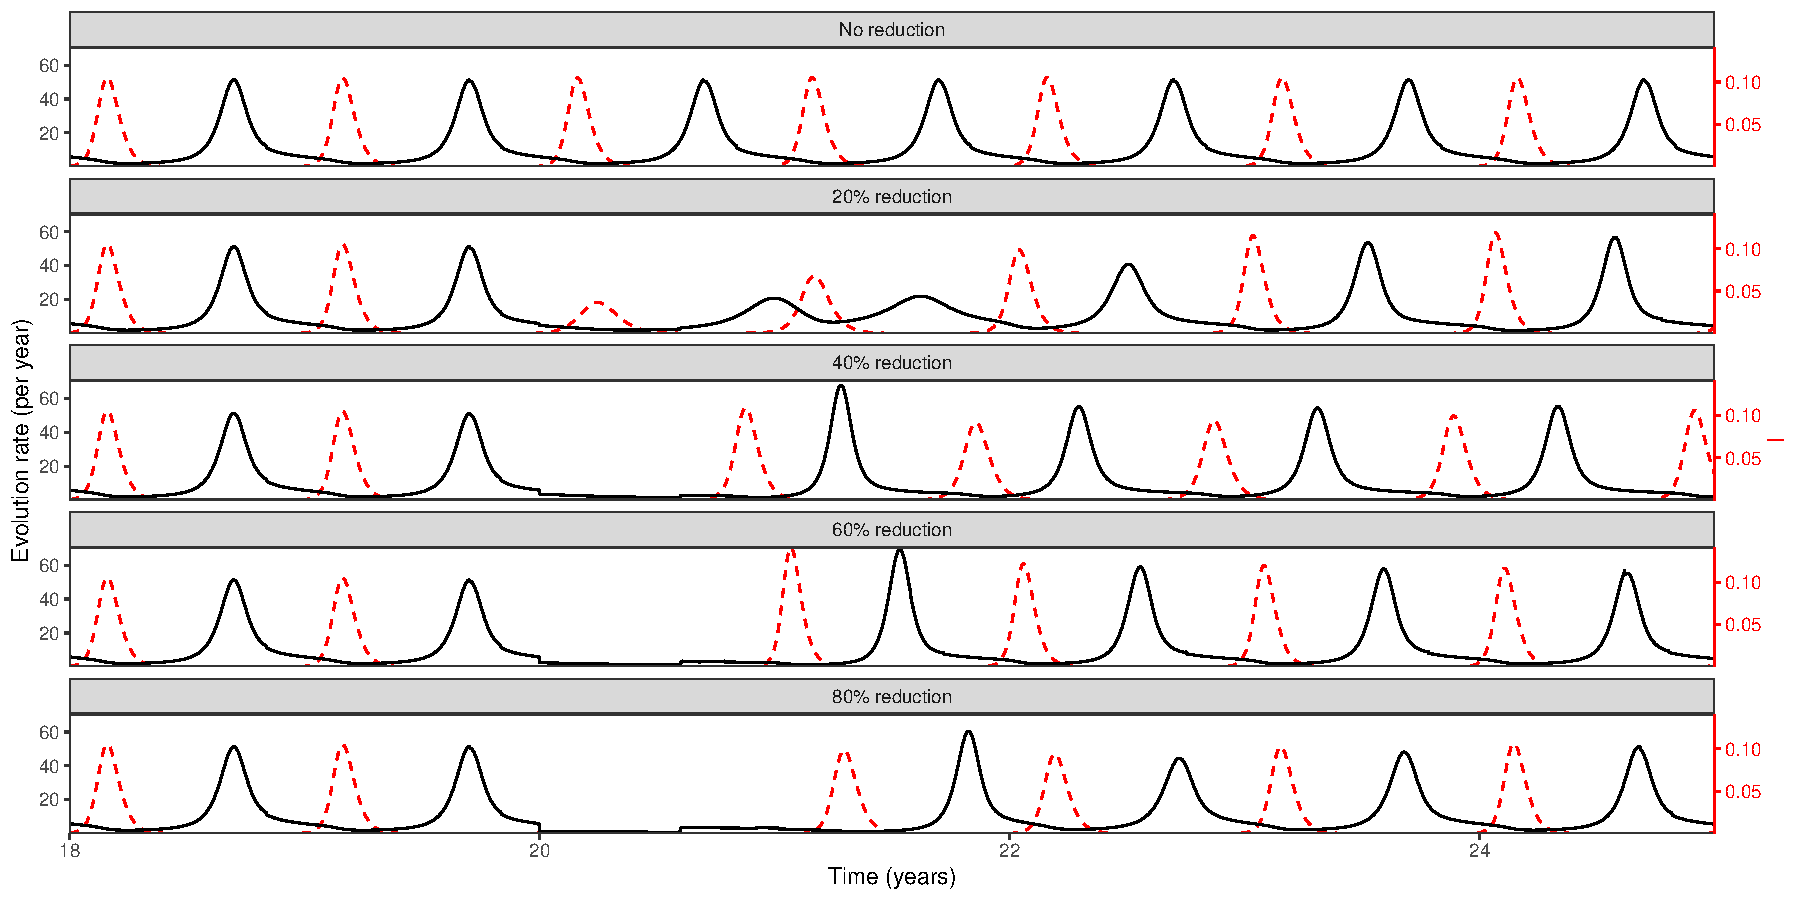
\includegraphics[width=\textwidth]{../figure/figure_flu_ode_6month_5.pdf}
\caption{
\textbf{Impact of reduction in transmission rate on evolution rate.}
Black lines represent the rate of evolution, which we define as the rate at which the mean strain number changes.
Red lines represent total prevalence $I = \sum_j I_j$.
The trajectories of evolution rate closely resemble that of strain diversities, shown in Figure 3.
The main difference is that this figure clearly illustrates that there is ``no'' evolution under strong intervention (evolution rate is roughly equal to 0).
}
\end{figure}


\pagebreak

\section{1 year control}

\begin{figure}[!h]
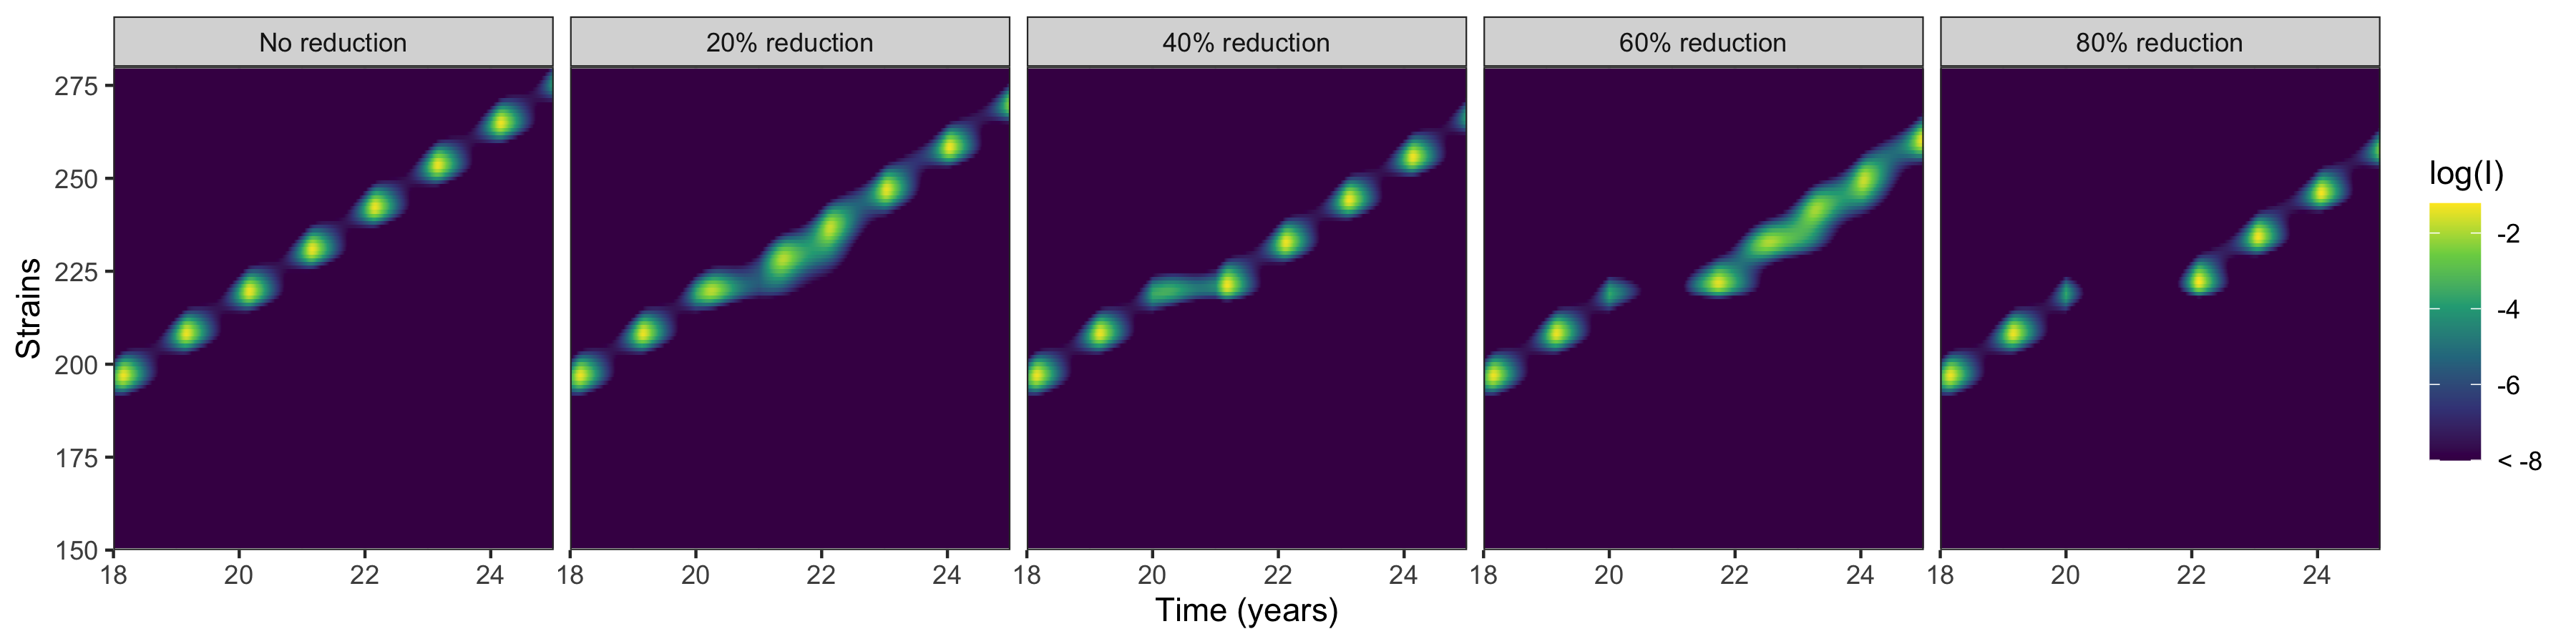
\includegraphics[width=\textwidth]{../figure/figure_flu_ode_1year_1.pdf}
\caption{
\textbf{Impact of reduction in transmission rate on epidemic dynamics.}
See Figure 1 for detailed caption.
Once again, we see interesting transient dynamics at $20\%$ and $60\%$ reduction.
}
\end{figure}

\pagebreak

\begin{figure}[!h]
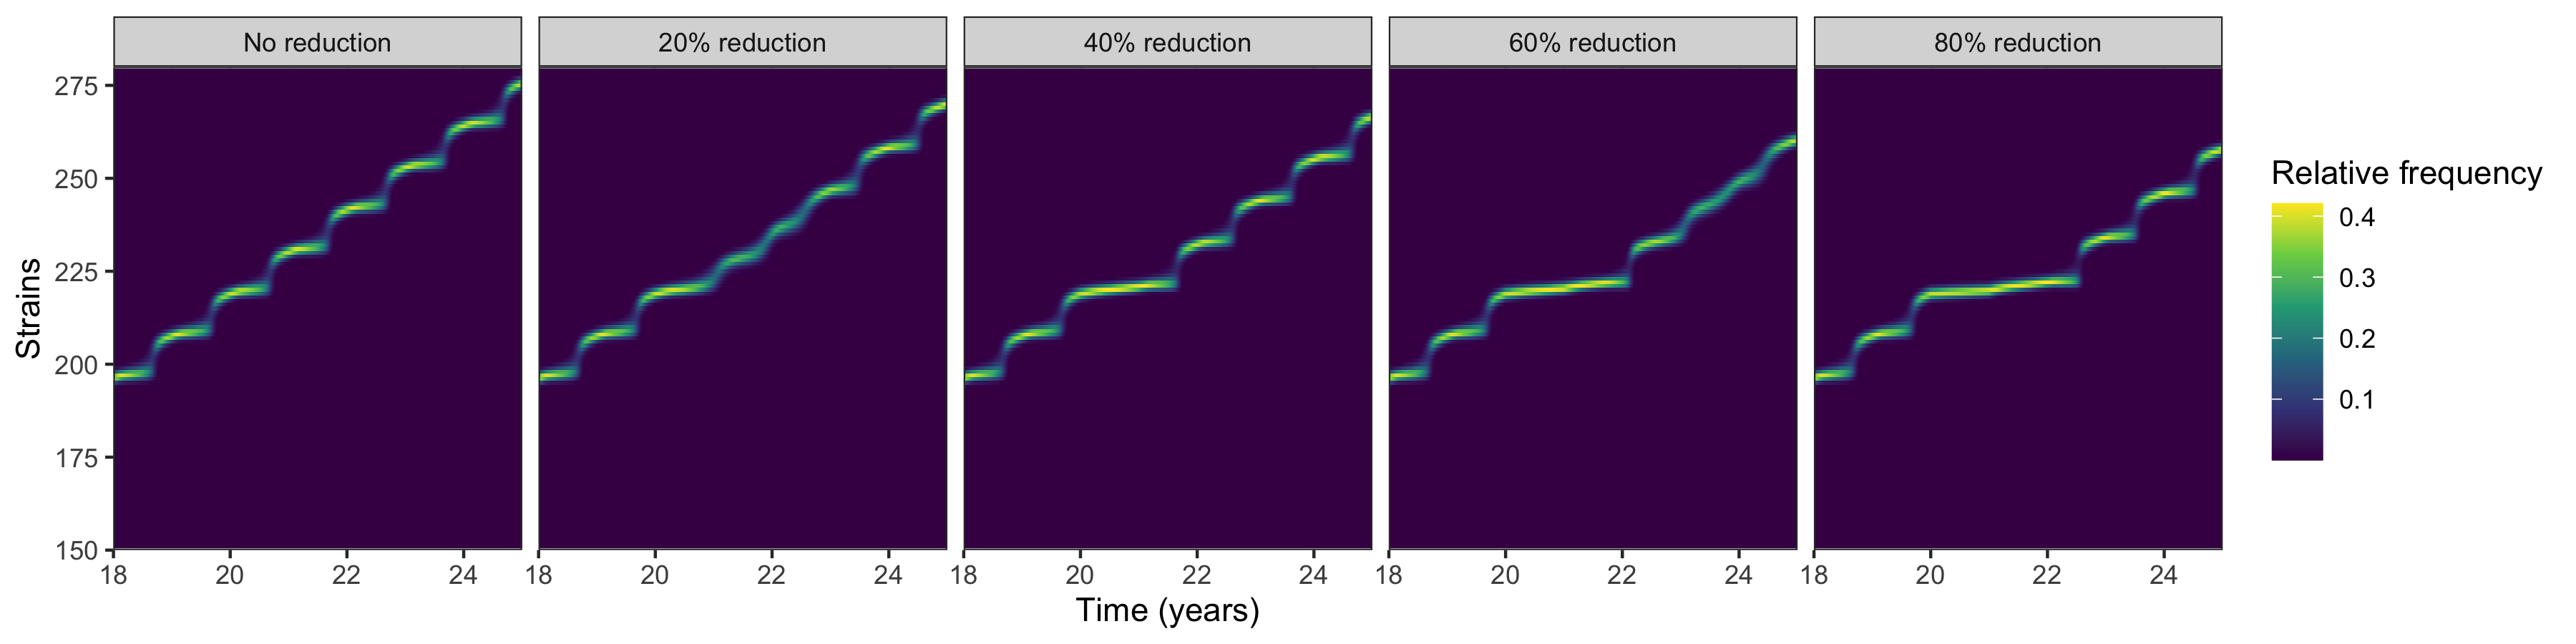
\includegraphics[width=\textwidth]{../figure/figure_flu_ode_1year_2.pdf}
\caption{
\textbf{Impact of reduction in transmission rate on epidemic dynamics.}
See Figure 2 for detailed caption.
}
\end{figure}

\pagebreak

\begin{figure}[!h]
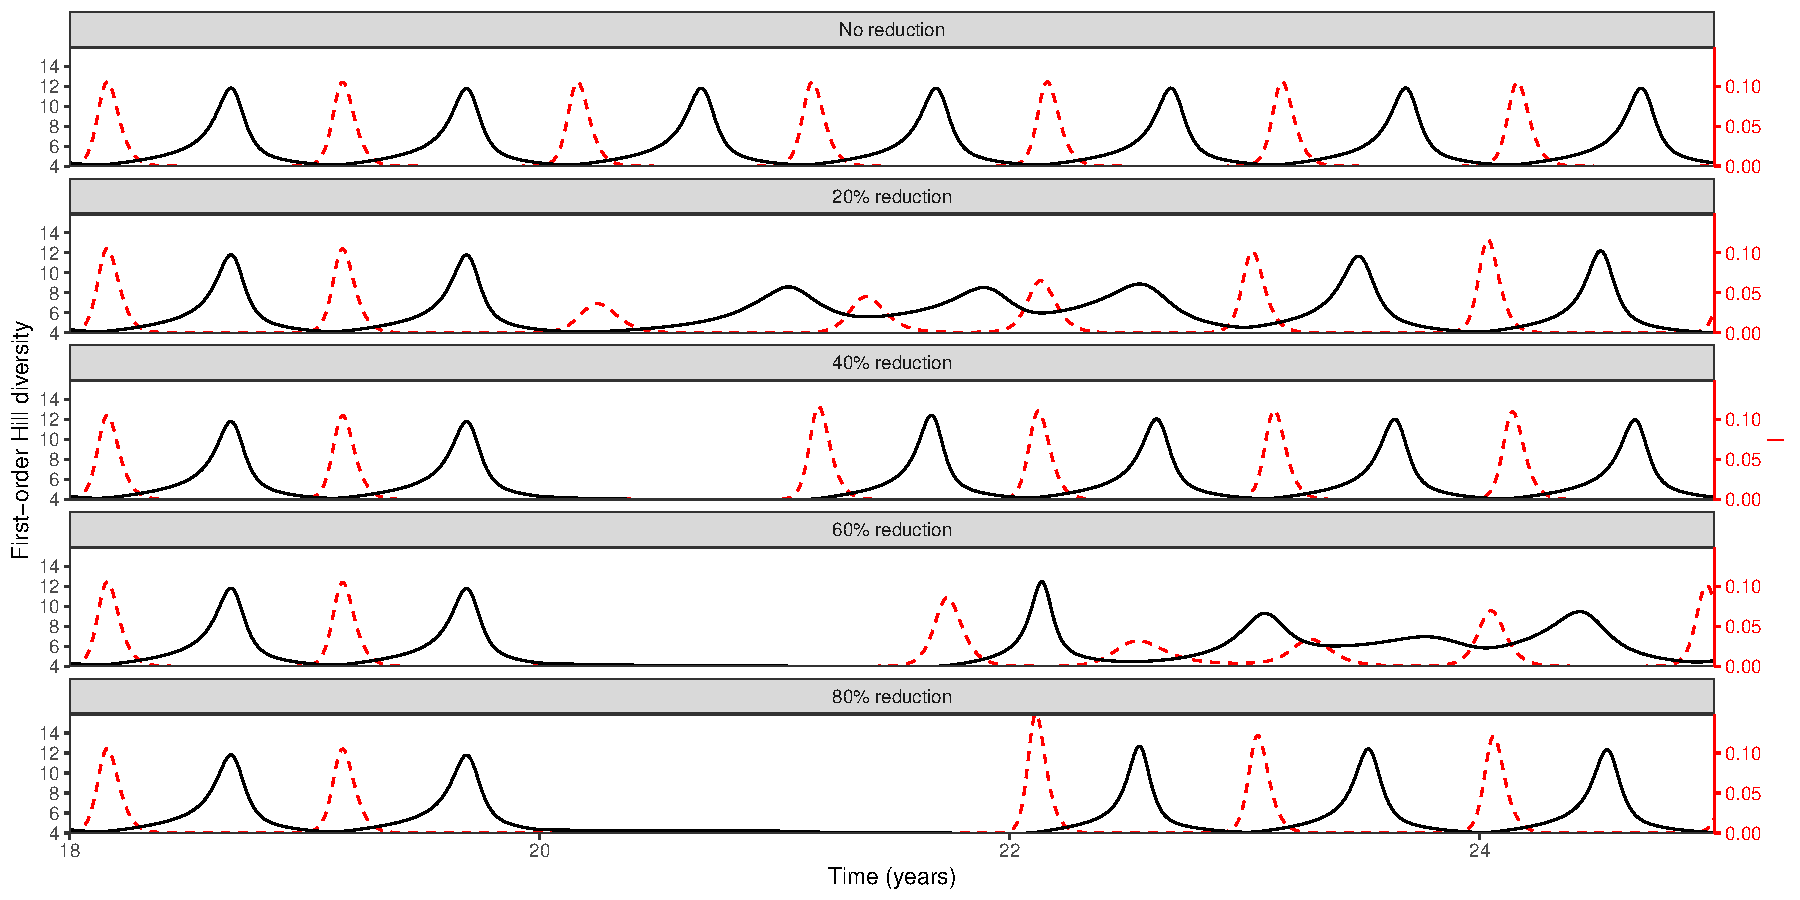
\includegraphics[width=\textwidth]{../figure/figure_flu_ode_1year_4.pdf}
\caption{
\textbf{Impact of reduction in transmission rate on epidemic dynamics.}
See Figure 3 for detailed caption.
Longer control does not necessarily lead to a bigger epidemic in this case because we do not explicitly model waning immunity.
In particular, we can get much smaller epidemics during off-seasons.
In practice, stochasticity and invasion from external sources are likely to play important roles in when the next epidemic occurs.
}
\end{figure}

\pagebreak

\begin{figure}[!h]
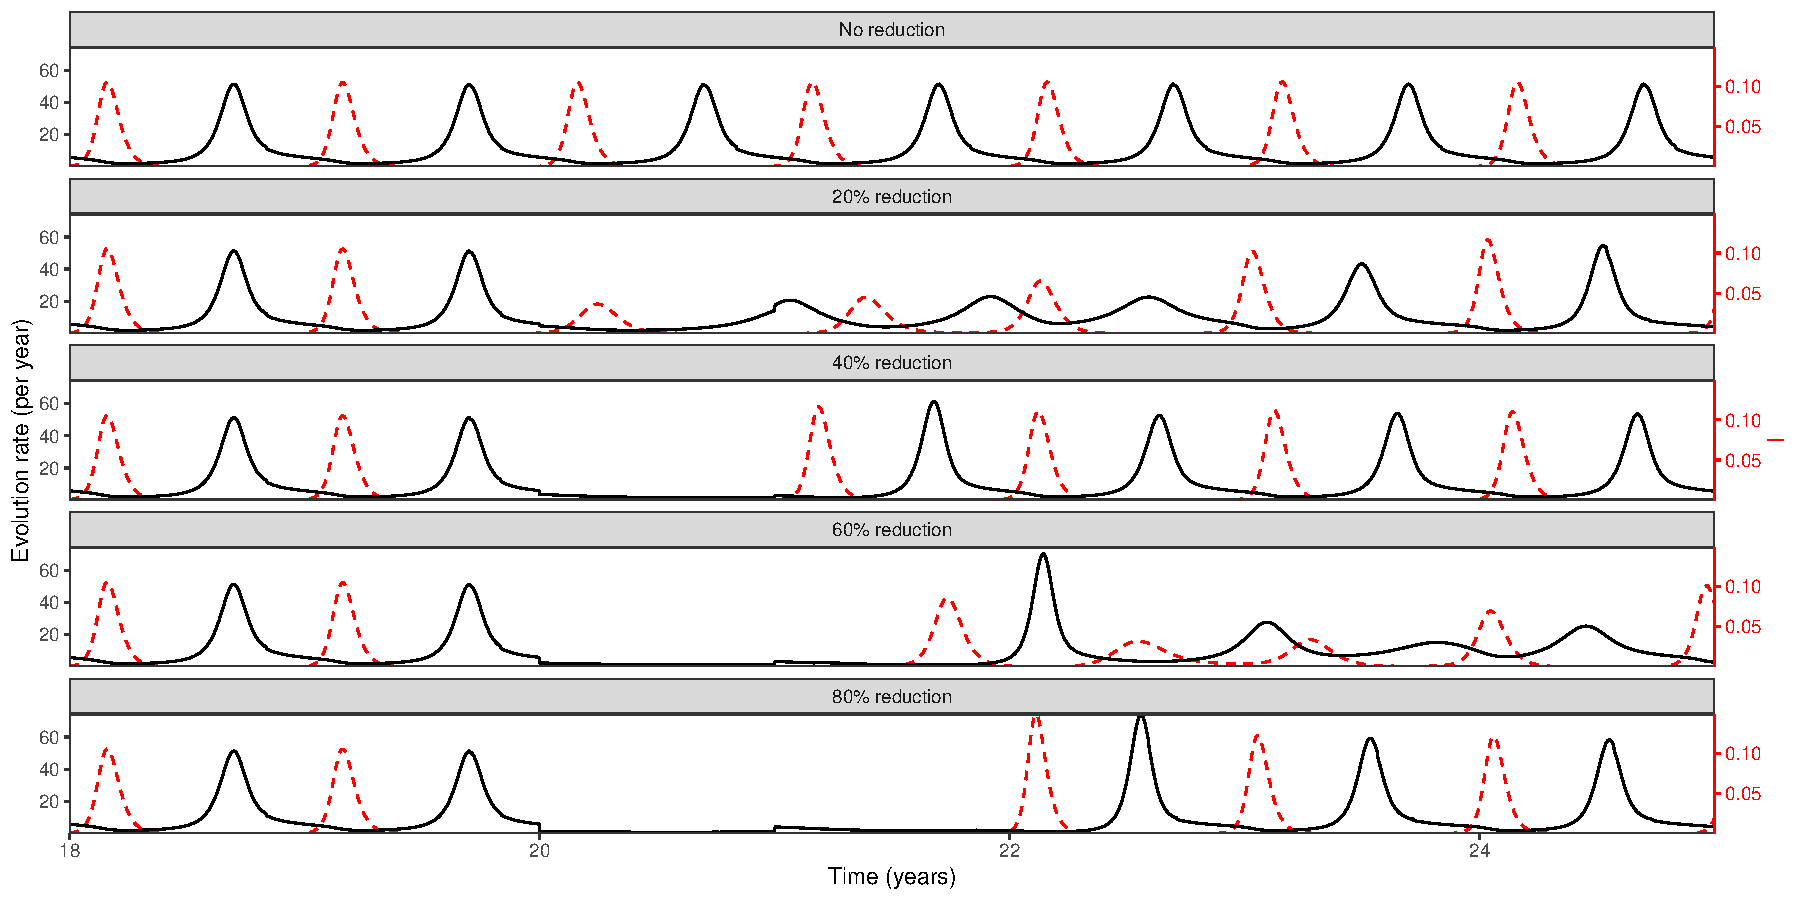
\includegraphics[width=\textwidth]{../figure/figure_flu_ode_1year_5.pdf}
\caption{
\textbf{Impact of reduction in transmission rate on epidemic dynamics.}
See Figure 4 for detailed caption.
}
\end{figure}

\pagebreak

\bibliography{flu}

\end{document}
